% This is a LaTeX template
% for preparing documents for DCCN
%
\documentclass[60x84/16,10pt]{dccn}

\usepackage[cp1251]{inputenc}

\usepackage{amsthm}

\newtheorem{theorem}{Theorem}[section]


% Don't remove definition.tex
\usepackage[T1,T2A]{fontenc}
\usepackage{ucs}
%\usepackage[utf8x]{inputenc}
\usepackage[english,russian]{babel}

%%  math extension packages

\usepackage{amsmath}
\usepackage{amssymb}
\usepackage{amscd}

\usepackage{mathtools}
\mathtoolsset{
showonlyrefs=true,
mathic=true,
}

\allowdisplaybreaks

%% graphic packages

\usepackage{graphicx}
\usepackage{epstopdf}

%% hyperref

\usepackage{hyperref}
\hypersetup{backref,
 colorlinks=false}
\hypersetup{pdfborder=0 0 0}

%% local definitions

\geometry{twoside}
\geometry{bindingoffset=0pt}

\geometry{includehead}
\geometry{hmargin={16mm,16mm},vmargin={12mm,13mm}}
\geometry{marginparwidth=0pt,marginparsep=0pt}
\geometry{headheight=0pt}
\geometry{headsep=\baselineskip}

\pagestyle{empty}

\usepackage{cite}


\begin{document}

{\selectlanguage{english}

\udc{519.218.31}

\title{Primary input flows in a tandem under prolongable cyclic service}

\author[1]{V. M. Kocheganov}
\author[1]{A. V. Zorine}

\address[1]{
N.I. Lobachevsky National Research\\  State University of Nizhny Novgorod\\
Gagarina av. 23, Nizhny Novgorod, 603950, Russia}

\begin{abstract}
 A tandem of queuing systems is under investigation. There are high and low-priority input flows in each system. Customers of the first system are serviced in the class of cyclic algorithms. After service high-priority customers of the first system are transferred to the second one. In the second system, customers are serviced in the class of cyclic algorithms with prolongations. This means low-priority customers are serviced once their number exceeds predefined threshold. A mathematical model is constructed in form of a multidimensional denumerable discrete-time Markov chain. The queues of primary input flows are of special interest in this paper. Partial generating functions of two-dimensional Markov chain are found. Sufficient condition for steady state existence is also given.
\end{abstract}

{\sloppy
\keywords{tandem of controlling queuing systems, cyclic algorithm with prolongations, conflicting flows, multidimensional denumerable discrete-time Markov chain.}
}


\maketitle 

\section{Introduction}
\label{sec:intro}
There is a lot of literature dedicated to conflicting traffic flows control at crossroad. One can find following types of algorithms investigated there: cyclic algorithm with a loop, cyclic algorithm with changing regimes, fixed duration cyclic algorithm, etc. See~\cite{n:f:p:1968,f:1977,l:f:2000,p:f:2008,a:b:2010}. Though this is almost always the case, when after vehicle passes one crossroad, it finds itself on another. That is in a real life there are more than one crossroad on the way. In other words, an output flow of cars from
the first intersection forms an input flow of cars of the next intersection. This imposes that the second input flow
no longer has an \textit{a priori} known simple probabilistic structure (for example, a
non-ordinary Poison flow), and knowledge about the service algorithm should be taken into account to deduce formation conditions of the first output flow.

Tandems of crossroads are studied for example in the following papers. In~\cite{z:2012} a mathematical model of two intersections in tandem governed by cyclic algorithms was investigated and stability conditions were found.
In~\cite{y:l:1985} a computer-aided
simulation of adjacent intersections was carried out.  In this paper we assume that the first intersection is governed by a cyclic algorithm while the second intersection is governed by a cyclic algorithm with prolongations. The high priority input flow of the first system and low priority input flow of the second system we will call primary input flows. This is because they are both generated by the environment and not by the system as the secondary input flows. The queues of primary input flows  take central place in this paper. This work continues studying in \cite{k:z:2016} and \cite{k:z:2016:2}.

\section{The problem settings} 
\label{sec:base-section}
Consider a queuing system with a scheme shown in Fig.~\ref{SystemScheme}.  
\begin{figure}[b]
   \centering
    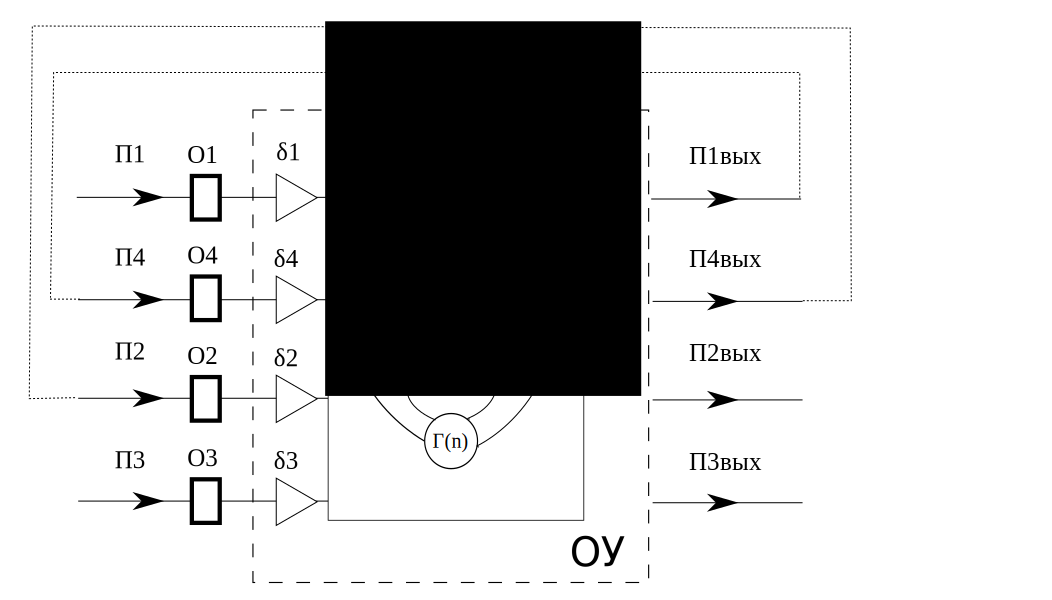
\includegraphics[width=\textwidth]{SystemScheme.pdf} % or {1.eps} in case of EPS format of the picture
    \caption {Scheme of the queuing system as a cybernetic control system}
    \label{SystemScheme}
\end{figure}
There are four
input flows of customers $\Pi_1$, $\Pi_2$, $\Pi_3$, and $\Pi_4$ entering the single server queueing
system. Customers in the input flow $\Pi_j$, $j \in \{1,2,3,4\}$ join a queue $O_j$ with an
unlimited capacity. For $j \in \{1,2,3\}$ the discipline of the queue $O_j$ is FIFO (First In First
Out). Discipline of the queue $O_4$ will be described later. The input flows $\Pi_1$ and $\Pi_3$ are
generated by an external environment, which has only one state. Each of these flows is a nonordinary
Poisson flow. Denote by $\lambda_1$ and $\lambda_3$ the intensities of bulk arrivals for the flows
$\Pi_1$ and $\Pi_3$ respectively. The probability generating function of number of customers in a
bulk in the flow $\Pi_j$ is $f_j(z) = \sum_{\nu=1}^{\infty} p_{\nu}^{(j)} z ^{\nu}, \quad j\in \{1,3\}.$

We assume that $f_j(z)$ converges for any $z\in \mathbb{C}$ such that $|z|<(1+\varepsilon)$,
$\varepsilon>0$. Here $p_{\nu}^{(j)}$ is the probability of a bulk size in flow $\Pi_j$ being
exactly $\nu=1$, $2$, \ldots. Having been serviced the customers from $O_1$ come back to the system
as the $\Pi_4$ customers. The $\Pi_4$ customers in turn after service enter the system as the
$\Pi_2$ ones. The flows $\Pi_2$ and $\Pi_3$ are conflicting in the sense that their customers can't
be serviced simultaneously. This implies that the problem can't be reduced to a problem with fewer
input flows by merging the flows together.


In order to describe the server behavior positive integers $d$, $n_0$, $n_1$, $\ldots$,
$n_d$ are fixed and a finite set $\Gamma=\{\Gamma^{(k,r)} \colon k=0,1,\ldots,d; r=1,2,\ldots
n_k\}$ of states server can reside in is introduced. At the state $\Gamma^{(k,r)}$ the server stays during a constant 
time $T^{(k,r)}$. We will assume, that for each fixed $k^*$ cycle subset $\{\Gamma^{(k^*,r)} \colon r=1,2,\ldots
n_k^*\} = C_{k^*}^{\mathrm{N}} \cup  C_{k^*}^{\mathrm{O}} \cup  C_{k^*}^{\mathrm{I}}$, that is consists of three disjoint sets called neutral, output and input sets of states.  In more details server is described in~\cite{k:z:2016:2}.

In general, service durations of different customers can be dependent and may have different laws of
probability distributions. So, saturation flows will be used to define the service process. A
saturation flow $\Pi^{\mathrm{\text{sat}}}_j$, $j \in \{1,2,3,4\}$, is defined as a virtual output
flow under the maximum usage of the server and unlimited number of customer in the queue $O_j$. The
saturation flow $\Pi^{\mathrm{\text{sat}}}_j$, $j\in \{1,2,3\}$ contains a non-random number
$\ell({k,r,j)}\geqslant0$ of customers in the server state $\Gamma^{(k,r)}$.

A real-life example of just described queuing system is a tandem of two consecutive crossroads
(Fig. \ref{crossroads}).
\begin{figure}[b]
   \centering
    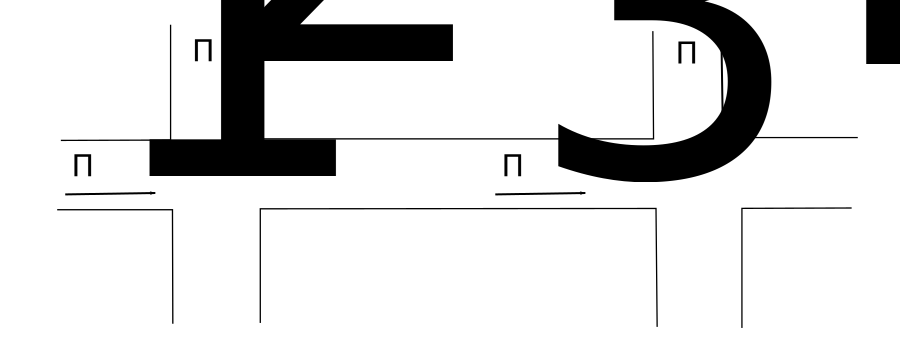
\includegraphics[width=\textwidth]{Crossroads.pdf} 
    \caption {A tandem of crossroads, the physical interpretation of the queuing system under study}
    \label{crossroads}
\end{figure}
The input flows are flows of vehicles. The flows $\Pi_1$ and $\Pi_5$ at the first crossroad are
conflicting; $\Pi_2$ and $\Pi_3$ at the second crossroad are also conflicting. Every vehicle from
the flow $\Pi_1$ after passing first road intersection joint the flow $\Pi_4$ and enters the queue
$O_4$. After some random time interval the vehicle arrives to the next road intersection. Such a pair
of crossroads is an instance of a more general queuing model described above.

\section{Mathematical model}
The queuing system under investigation can be regarded as a cybernetic control system that helps to
rigorously construct a formal stochastic model~\cite{z:2012}. The scheme of the control system is
shown in Fig.~\ref{SystemScheme}. There are following blocks present in the scheme: 1)~the external
environment with one state; 2) input poles of the first type~--- the input flows $\Pi_1$, $\Pi_2$,
$\Pi_3$, and $\Pi_4$; 3) input poles of the second type~--- the saturation flows
$\Pi^{\mathrm{\text{sat}}}_1$, $\Pi^{\mathrm{\text{sat}}}_2$, $\Pi^{\mathrm{\text{sat}}}_3$, and
$\Pi^{\mathrm{\text{sat}}}_4$; 4)~an external memory~--- the queues $O_1$, $O_2$, $O_3$, and $O_4$;
5)~an information processing device for the external memory~--- the queue discipline units
$\delta_1$, $\delta_2$, $\delta_3$, and $\delta_4$; 6) an internal memory --- the server (OY); 7)~an
information processing device for internal memory~--- the graph of server state transitions;
8)~output poles~--- the output flows $\Pi^{\mathrm{\text{out}}}_1$, $\Pi^{\mathrm{\text{out}}}_2$,
$\Pi^{\mathrm{\text{out}}}_3$, and $\Pi^{\mathrm{\text{out}}}_4$.  The coordinate of a block is
its number on the scheme.

Let us  introduce the following variables and elements along with their
value ranges. To fix a discrete time scale consider the epochs $\tau_0=0$, $\tau_1$, $\tau_2$,
$\ldots$ when the server changes its state. Let $\Gamma_i\in\Gamma$ be the server state
during the interval $(\tau_{i-1};\tau_i]$, $\varkappa_{j,i} \in \mathbb{Z}_+ $ be the number of customers in
the queue $O_j$ at the instant $\tau_i$, $\eta_{j,i} \in \mathbb{Z}_+$ be the number of customers
arrived into the queue $O_j$ from the flow $\Pi_j$ during the interval $(\tau_{i};\tau_{i+1}]$, $\xi_{j,i} \in
\mathbb{Z}_+$ be the number of customers in the saturation flow $\Pi^{\mathrm{\text{sat}}}_j$ during
the interval $(\tau_{i};\tau_{i+1}]$, $\overline{\xi}_{j,i}\in \mathbb{Z}_+$ be the actual number of 
serviced customers from the queue  $O_j$ during the interval $(\tau_{i};\tau_{i+1}]$, $j\in
\{1,2,3,4\}$.

The server changes its state according to the following rule:
%\begin{equation}
$
\Gamma_{i+1}=h(\Gamma_i,\varkappa_{3,i})
$
%\label{gammaFunc}
%\end{equation}
where the mapping $h(\cdot,\cdot)$ is defined in paper \cite{k:z:2016:2}.

Let $\varphi_1(\cdot,\cdot)$ and $\varphi_3(\cdot,\cdot)$ be defined by series expansions
\begin{equation*}
\sum_{\nu=0}^{\infty} z^\nu\varphi_j(\nu,t) = \exp\{\lambda_j t (f_j(z)-1)\},
\end{equation*}
$j \in \{1,3\}$. The function
$\varphi_j(\nu,t)$ equals the probability of  $\nu=0$, $1$, $\ldots${} arrivals in the flow
$\Pi_j$ during time $t \geqslant 0$. If $\nu < 0$ the value of $\varphi_j(\nu,t)$ is set to
zero.

Mathematical model in more details can be found in work \cite{k:z:2016}. From
now on we focus on primary input flows customers in the queues $O_1$ and~$O_3$.

\section{The queues of primary input flows}
Here we will consider the stochastic sequence
\begin{equation}
\label{eq:theMC}
\{(\Gamma_i(\omega), \varkappa_{1,i}(\omega),\varkappa_{3,i}(\omega)); i =0, 1, \ldots\},
\end{equation}
which includes the number of customers $\varkappa_{1, i}(\omega)$ and $\varkappa_{3, i}(\omega)$ in the queues $O_1$ and $O_3$ respectfully.  In this
section we will report several results concerning this stochastic sequence.


Let's define for $\gamma \in \Gamma$ and $(x_1, x_3) \in Z^2_+$ values
\begin{equation*}
Q_{1,i}(\gamma,x_1,x_3) = {\mathbf P}(\{\omega\colon \Gamma_{i}(\omega)=\gamma, \varkappa_{1,i}(\omega)=x_1, \varkappa_{3,i}(\omega)=x_3\}).
\end{equation*}

Suppose $k$ and $r$ are such that $\Gamma^{(k,r)}\in \Gamma$. Let's define  partial probability generating functions 
\begin{equation*}
\mathfrak{M}^{(1,i)}(k,r,v_1,v_3) = \sum_{w_1=0}^{\infty}\sum_{w_3=0}^{\infty} Q_{1,i}(\Gamma^{(k,r)},w_1,w_3) v_1^{w_1} v_3^{w_3},
\end{equation*}
and auxilary functions
\begin{align*}
q^{(1,i)}(k,r, v_1) &= v_1^{-\ell(k,r,1)}\sum_{w=0}^{\infty} \varphi_1(w,T^{(k,r)})v_1^w;\\
q^{(3,i)}(k,r, v_3) &= q_{k,r} (v_3) = v_3^{-\ell(k,r,3)}\sum_{w=0}^{\infty} \varphi_3(w,T^{(k,r)})v_3^w,
\end{align*}
and 
\begin{multline*}
    g^{(1,i)}(k,r,v_1,v_3) =\sum_{x_3=L+1}^{\infty} \sum_{x_1=\ell(k,r,1)+1}^{\infty}  [  Q_{1,i}(\Gamma^{(k, r\ominus_{k}1)},x_1, x_3) +\\+Q_{1,i}(\Gamma^{(0, r_2)},x_1, x_3)]v_1^{x_1} v_3^{ x_3}, \quad \Gamma^{(k,r)} \in C_{k}^{\mathrm{I}}
\\
g^{(1,i)}(k,r,v_1,v_3) =\\
    =\!\!\sum_{x_3=\ell(k,r,3)+1}^{\infty} \sum_{x_1=\ell(k,r,1)+1}^{\infty}
    \!\! Q_{1,i}(\Gamma^{(k, r\ominus_{k}1)}\!,x_1, x_3) v_1^{x_1} v_3^{ x_3}, \; \Gamma^{(k,r)} \in C_{k}^{\mathrm{O}} \cup C_{k}^{\mathrm{N}}
\end{multline*}
We also introduce residuals $\alpha^{(1,i)}(k,r,v_1,v_3)$:
\begin{multline*}
\alpha^{(1,i)}(k,r,v_1,v_3) = 
    \sum_{x_3=0}^{\ell(k,r,3)}\sum_{w_3=1}^{\infty} \sum_{w_1=1}^{\infty} \sum_{x_1=0}^{w_1+\ell(k,r,1)}  [  Q_{1,i}(\Gamma^{(k_1, r_1)},x_1, x_3)
    +\\+Q_{1,i}(\Gamma^{(0, r\ominus_0 1)},x_1, x_3)]
   \times \varphi_3(w_3 + \ell(k,r,3) - x_3,T^{(k,r)})  \times \\ \times \varphi_1(w_1 + \ell(k,r,1) - x_1,T^{(k,r)})  \times v_1^{w_1} v_3^{w_3} + q^{(3,i)}(k,r,v_3) \times\\
    \times  \sum_{x_1=0}^{\ell(k,r,1)}\sum_{x_3=\ell(k,r,3)+1}^{L} v_3^{x_3} \sum_{w_1=1}^{\infty}    [  Q_{1,i}(\Gamma^{(k_1, r_1)},x_1, x_3) + \displaybreak[0]\\
    +Q_{1,i}(\Gamma^{(0, r\ominus_0 1)},x_1, x_3)] \varphi_1(w_1 + \ell(k,r,1) - x_1,T^{(k,r)})v_1^{w_1} +  \displaybreak[0]\\
    +q^{(1,i)}(k,r,v_1) q^{(3,i)}(k,r,v_3)\sum_{x_3=\ell(k,r,3)+1}^{L} \sum_{x_1=\ell(k,r,1)+1}^{\infty}    [  Q_{1,i}(\Gamma^{(k_1, r_1)},x_1, x_3) +\\
    +Q_{1,i}(\Gamma^{(0, r\ominus_0 1)},x_1, x_3)] v_1^{x_1} v_3^{ x_3} 
    +  \sum_{x_1=0}^{\ell(k,r,1)} \sum_{x_3=0}^{\ell(k,r,3)} [  Q_{1,i}(\Gamma^{(k_1, r_1)},x_1, x_3) +\\
    +Q_{1,i}(\Gamma^{(0, r\ominus_0 1)},x_1, x_3)]\times
\sum_{a=0}^{\ell(k,r,3)-x_3}\varphi_3(a,T^{(k,r)}) \times \sum_{a=0}^{\ell(k,r,1)-x_1}\varphi_1(a,T^{(k,r)})
+ \\ +
    \sum_{w_3=1}^{\infty} \sum_{x_1=0}^{\ell(k,r,1)} \sum_{x_3=0}^{\min{\{L, w_3 + \ell(k,r,3)\}}} [  Q_{1,i}(\Gamma^{(k_1, r_1)},x_1, x_3) +\\
    +Q_{1,i}(\Gamma^{(0, r\ominus_0 1)},x_1, x_3)] \times \varphi_3(w_3 + \ell(k,r,3) - x_3,T^{(k,r)})  \times\\ \times \sum_{a=0}^{\ell(k,r,1)-x_1}\varphi_1(a,T^{(k,r)})  v_3^{w_3}
    +
     \sum_{w_1=1}^{\infty} \sum_{x_1=0}^{w_1 + \ell(k,r,1) } \sum_{x_3=0}^{\ell(k,r,3)} [  Q_{1,i}(\Gamma^{(k_1, r_1)},x_1, x_3) +\\
    +Q_{1,i}(\Gamma^{(0, r\ominus_0 1)},x_1, x_3)] \times \sum_{a=0}^{\ell(k,r,3)-x_3}\varphi_3(a,T^{(k,r)}) \times\\ \times \varphi_1(w_1 + \ell(k,r,1) - x_1,T^{(k,r)}) v_1^{w_1} 
    , \quad k = 0.
\end{multline*}
Residuals for input states $\Gamma^{(k,r)} \in C_{k}^{\mathrm{I}}$ look as follows:
\begin{multline*}
\alpha^{(1,i)}(k,r,v_1,v_3) = 
     q^{(3,i)}(k,r,v_3) \times\\
    \times  \sum_{x_1=0}^{\ell(k,r,1)}\sum_{x_3=L}^{\infty}  v_3^{x_3} \sum_{w_1=1}^{\infty} [Q_{1,i}(\Gamma^{(0,r_2)},x_1, x_3)+Q_{1,i}(\Gamma^{(k,r\ominus_k 1)},x_1, x_3)]\times \\ \times \varphi_1(w_1 + \ell(k,r,1) - x_1,T^{(k,r)})v_1^{w_1} + \\
   \!+\!\!
    \sum_{w_3=L -\ell(k,r,3) + 1}^{\infty}\!\! \sum_{x_1=0}^{\ell(k,r,1)}
    \sum_{x_3=L+1}^{w_3 + \ell(k,r,3)}\!\!\!\!\![Q_{1,i}(\Gamma^{(0,r_2)}\!,x_1,
    x_3)\!+\!Q_{1,i}(\Gamma^{(k,r\ominus_k 1)}\!,x_1, x_3)] \!\times  \\ 
    \times \varphi_3(w_3 + \ell(k,r,3) - x_3,T^{(k,r)})  \times \sum_{a=0}^{\ell(k,r,1)-x_1}\varphi_1(a,T^{(k,r)})  v_3^{w_3} .
\end{multline*}
And residuals for output and neutral states $\Gamma^{(k,r)}\! \in C_{k}^{\mathrm{O}} \!\cup\! C_{k}^{\mathrm{N}}$:
\begin{multline*}
\alpha^{(1,i)}(k,r,v_1,v_3) = 
    \sum_{x_3=0}^{\ell(k,r,3)}\sum_{w_3=1}^{\infty} \sum_{w_1=1}^{\infty} \sum_{x_1=0}^{w_1+\ell(k,r,1)}  Q_{1,i}(\Gamma^{(k,r\ominus_k 1)},x_1, x_3) \times  \\
   \times \varphi_3(w_3 + \ell(k,r,3) - x_3,T^{(k,r)})   \varphi_1(w_1 + \ell(k,r,1) - x_1,T^{(k,r)})  v_1^{w_1} v_3^{w_3} + \\ + q^{(3,i)}(k,r,v_3) 
    \times  \sum_{x_1=0}^{\ell(k,r,1)}\sum_{x_3=\ell(k,r,3)+1}^{\infty}
    v_3^{x_3} \sum_{w_1=1}^{\infty}  Q_{1,i}(\Gamma^{(k,r\ominus_k 1)},x_1,
    x_3)\times \\ 
    \times \!\varphi_1(w_1 + \ell(k,r,1) - x_1,T^{(k,r)})v_1^{w_1} 
   +\!\!\!\sum_{x_1=0}^{\ell(k,r,1)} \sum_{x_3=0}^{\ell(k,r,3)} \!Q_{1,i}(\Gamma^{(k,r\ominus_k 1)},x_1, x_3)\!\times \\ \times
\sum_{a=0}^{\ell(k,r,3)-x_3}\varphi_3(a,T^{(k,r)}) \times \sum_{a=0}^{\ell(k,r,1)-x_1}\varphi_1(a,T^{(k,r)})
+ \\ + 
    \sum_{w_3=1}^{\infty} \sum_{x_1=0}^{\ell(k,r,1)} \sum_{x_3=0}^{w_3 + \ell(k,r,3)} Q_{1,i}(\Gamma^{(k,r\ominus_k 1)},x_1, x_3) \times  \\ \times \varphi_3(w_3 + \ell(k,r,3) - x_3,T^{(k,r)})  \times \sum_{a=0}^{\ell(k,r,1)-x_1}\varphi_1(a,T^{(k,r)})  v_3^{w_3} + \\
    +
    \sum_{w_1=1}^{\infty} \sum_{x_1=0}^{w_1 + \ell(k,r,1) } \sum_{x_3=0}^{\ell(k,r,3)} Q_{1,i}(\Gamma^{(k,r\ominus_k 1)},x_1, x_3) \times  \\ \times \!\sum_{a=0}^{\ell(k,r,3)-x_3}\!\!\varphi_3(a,T^{(k,r)})  \varphi_1(w_1 + \ell(k,r,1) - x_1,T^{(k,r)}) v_1^{w_1}.
\end{multline*}


\begin{theorem}
Following recurrent w.r.t. $i
\geqslant 0$ relations take place for the  partial probability generating functions:
\begin{enumerate}

\item $ \Gamma^{(0,\tilde{r})} \in \Gamma$, $\tilde{r} = \overline{1,n_0}$ 
$$
\mathfrak{M}^{(1,i+1)}(0,\tilde{r},v) = \alpha^{(1,i)}(0,\tilde{r},v_1,v_3);
$$
\item $\Gamma^{(\tilde{k},\tilde{r})} \in C_{\tilde{k}}^{\mathrm{I}} \cup C_{\tilde{k}}^{\mathrm{O}} \cup C_{\tilde{k}}^{\mathrm{N}}$
\begin{multline*}
\mathfrak{M}^{(1,i+1)}(\tilde{k},\tilde{r},v) = q^{(1,i)}(\tilde{k},\tilde{r},v_1) q^{(3,i)}(\tilde{k},\tilde{r},v_3) \times g^{(1,i)}(\tilde{k},\tilde{r},v_1,v_3)
     +\\+ \alpha^{(1,i)}(\tilde{k},\tilde{r},v_1,v_3);
\end{multline*}
\end{enumerate}

\label{theorem:gen}
\end{theorem}



\begin{theorem}\sloppy
For Markov chain~\eqref{eq:theMC} to have a stationary distribution $Q_1(\gamma,x)$, $(\gamma,x)\in \Gamma \times {\mathbb Z}_+$ it is sufficient to satisfy the following inequality 
\begin{equation}
\min_{\substack{k=\overline{1,d}\\ j=1,3}} { \frac{\sum_{r = 1}^{n_k} \ell(k,r,j) }{\lambda_j f_j'(1) \sum_{r=1}^{n_k} T^{(k,r)} }}>1.
\label{sufficient:double}
\end{equation}
\end{theorem}
For example, let the system have following characteristics: $\sum_{r} \ell(k,r,j) = 15$, $\sum_{r} T^{(k,r)}=60$, $\lambda_j=0.125$, $f_j'(1)=1.5$, $j\in \{1,3\}$, $k=\overline{1,d}$, $d=2$, $n_1=n_2=2$. In this case stationary distribution exists.

\section{Conclusion}
The tandem of queuing systems was considered. The problem settings are given and mathematical model was constructed in the form of multidimensional Markov chain $\{(\Gamma_i, \varkappa_{1,i}, \varkappa_{2,i}, \varkappa_{3,i}, \varkappa_{4,i}); i \geqslant 0\}$. The main result of this paper concerns Markov chain $\{(\Gamma_i, \varkappa_{1,i}, \varkappa_{3,i}); i \geqslant 0 \}$. Recurrent relations were found for the partial  probability generating functions, which in turn gives the basis for sufficient condition of stationary distribution existence findings. It is always very important to have the conditions under which the system can come into stable mode. In such stable mode more wide and detailed analysis can be done.

\begin{thebibliography}{11}
\bibitem{p:f:2008}%
  Proidakova E.V., Fedotkin M.A. Control of output flows in the system with cyclic servicing and
  readjustments~// Automation and remote control. 2008. V. 69, No. 6. P.~993--1002.
\bibitem{f:1977} %
Fedotkin M.~A. On a class of stable algorithms for control of conflicting flows or arriving
  airplanes~// Problems of control and information theory. 1977. V.~6, No.~1. P.~13--22.

\bibitem{l:f:2000}%
  Litvak N.~V., Fedotkin M.~A. A probabilistic model for the
  adaptive control of conflict flows~// Automation and Remote Control. 2000. V. 61, No. 5. P.~777--784.

  \bibitem{n:f:p:1968} Neimark Yu.~I., Fedotkin M.~A., Preobrazhenskaja A.~M. Operation of an automate
  with feedback controlling traffic at an intersection~// Izvestija of USSR Academy of Sciences,
  Technical Cybernetic. 1968. No.~5. P.~129--141.
\bibitem{a:b:2010}%
  Afanasyeva L.~G., Bulinskaya E.~V. Mathematical models of transport systems based on queueing
  theory~// Trudy of Moscow Institute of Physocs and Technology. 2010. No.~4. P.6--21. 
  \bibitem{z:2012}%
  Zorin A.V. Stability of a tandem of queueing systems with Bernoulli noninstantaneous transfer of
  customers~// Theory of Probability and Mathematical Statistics. 2012. V.~84. P.~173-188.
\bibitem{y:l:1985} %
  Yamada K., Lam T.~N. Simulation analysis of two adjacent traffic signals~// Proceedings of the
  17th winter simulation conference. ACM, New York. 1985. P.~454--464.
\bibitem{k:z:2016} %
Kocheganov~V.M., Zorine~A.V. Low-Priority Queue Fluctuations in Tandem of Queuing Systems Under Cyclic Control with Prolongations // Distributed Computer and Communication Networks. Ser. Communications in Computer and Information Science. 2016. V.~601. P.~268-279.
\bibitem{k:z:2016:2} %
Kocheganov~V.M., Zorine~A.V. Low-Priority Queue and Server's Steady-State Existence in a Tandem Under Prolongable Cyclic Service // Distributed Computer and Communication Networks. Ser. Communications in Computer and Information Science. Springer, Cham. 2016. V.~678. P.~210-221.
\end{thebibliography}

%% You may use bibtex.
% \bibliographystyle{gost2008l}
% \bibliography{dccn_template_en}

%\makealttitle

} %END \selectlanguage

\end{document}


